\documentclass{article}
\usepackage{tikz}
\usetikzlibrary{positioning}
\usetikzlibrary{calc}

%%
\usetikzlibrary{shapes.geometric, arrows, positioning}

\tikzstyle{process} = [rectangle, rounded corners, minimum width=2.5cm, minimum height=1cm, draw=black, fill=gray!10]
\tikzstyle{box} = [rectangle, minimum width=2cm, minimum height=1cm, draw=black]
\tikzstyle{arrow} = [thick,->,>=stealth]
\tikzstyle{textlabel} = [align=center]

%%

\begin{document}

\title{TikZ Graph Example}
\author{Your Name}
\date{\today}

\maketitle

\section{Introduction}
This is an example document to create TikZ graphs.

\section{Previous CAG TikZ Graph}
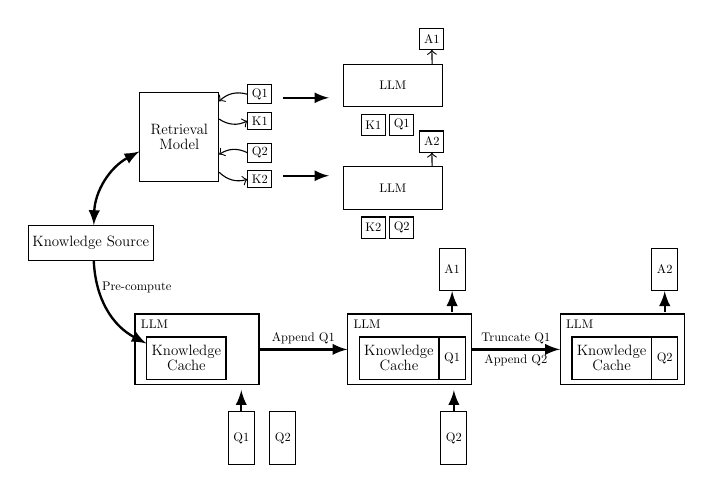
\begin{tikzpicture}[scale=0.45, transform shape]
    % Your TikZ code goes here
    \node[draw, box] at (0, 0) (knowledge) {\large Knowledge Source};
    \node[
        draw, box, text width=2cm, minimum height=2.5cm, minimum width=2cm, align=center
    ] at (2.5, 3) (retrieval_model) {\large Retrieval Model};
    % \node[draw, box] at (3, 1.5) (retrieval_model) {Retrieval Model};
    
    \draw[<->, latex-latex, line width=0.3mm, bend left] (knowledge) to (retrieval_model);
    
    % \draw[<->] (retrieval_model) to (knowledge_cache);
    
    \coordinate (retrieve_Q1) at ($(retrieval_model.east) + (0cm, 1cm)$);
    \coordinate (retrieve_K1) at ($(retrieval_model.east) + (0cm, 0.5cm)$);
    \coordinate (retrieve_Q2) at ($(retrieval_model.east) + (0cm, -0.5cm)$);
    \coordinate (retrieve_K2) at ($(retrieval_model.east) + (0cm, -1cm)$);
    
    \node (Q1) [draw, rectangle, right=0.8cm of retrieval_model, yshift=1.2cm] {Q1};
    \node (K1) [draw, rectangle, right=0.8cm of retrieval_model, yshift=0.45cm] {K1};
    \node (Q2) [draw, rectangle, right=0.8cm of retrieval_model, yshift=-0.45cm] {Q2};
    \node (K2) [draw, rectangle, right=0.8cm of retrieval_model, yshift=-1.2cm] {K2};
    
    \coordinate (Q1_left) at ($(Q1.west) + (0cm, 0cm)$);
    \coordinate (K1_left) at ($(K1.west) + (0cm, 0cm)$);
    \coordinate (Q2_left) at ($(Q2.west) + (0cm, 0cm)$);
    \coordinate (K2_left) at ($(K2.west) + (0cm, 0cm)$);

    \draw[<-, bend left] (retrieve_Q1) to (Q1_left);
    \draw[->, bend right] (retrieve_K1) to (K1_left);
    \draw[<-, bend left] (retrieve_Q2) to (Q2_left);
    \draw[->, bend right] (retrieve_K2) to (K2_left);

    \node (LLM1) [box, minimum height=1.2cm, minimum width=2.8cm, align=center, right=2cm of Q1, yshift=0.25cm] {LLM};
    \node (LLM2) [box, minimum height=1.2cm, minimum width=2.8cm, align=center, right=2cm of K2, yshift=-0.25cm] {LLM};
    
    \coordinate (LLM1_Arrow_start) at ($(retrieval_model.east) + (1.8cm, 1.1cm)$);
    \coordinate (LLM1_Arrow_end) at ($(retrieval_model.east) + (3.1cm, 1.1cm)$);
    \draw[-latex, thick] (LLM1_Arrow_start) to (LLM1_Arrow_end);

    \coordinate (LLM1_Arrow_start) at ($(retrieval_model.east) + (1.8cm, -1.1cm)$);
    \coordinate (LLM1_Arrow_end) at ($(retrieval_model.east) + (3.1cm, -1.1cm)$);
    \draw[-latex, thick] (LLM1_Arrow_start) to (LLM1_Arrow_end);


    \node (Q1) [draw, rectangle, minimum height=0.6cm, minimum width=0.4cm, below=0.2cm of LLM1, xshift=0.25cm] {Q1};
    \node (K1) [draw, rectangle, minimum height=0.6cm, minimum width=0.4cm, below=0.2cm of LLM1, xshift=-0.55cm] {K1};
    \node (A1) [draw, rectangle, minimum height=0.6cm, minimum width=0.4cm, above=0.4cm of LLM1, xshift=1.1cm] {A1};
    \coordinate (LLM1_right) at ($(LLM1.east) + (-0.3cm, 0.6cm)$);
    \draw[->] (LLM1_right) to (A1.south);

    \node (Q2) [draw, rectangle, minimum height=0.6cm, minimum width=0.4cm, below=0.2cm of LLM2, xshift=0.25cm] {Q2};
    \node (K2) [draw, rectangle, minimum height=0.6cm, minimum width=0.4cm, below=0.2cm of LLM2, xshift=-0.55cm] {K2};
    \node (A2) [draw, rectangle, minimum height=0.6cm, minimum width=0.4cm, above=0.4cm of LLM2, xshift=1.1cm] {A2};    
    \coordinate (LLM2_right) at ($(LLM2.east) + (-0.3cm, 0.6cm)$);
    \draw[->] (LLM2_right) to (A2.south);


    \node[
        draw, box, text width=2cm, minimum height=2cm, minimum width=3.5cm, align=center
    ] at (3, -3) (LLM1) {};
    \node at ($(LLM1) + (-1.2cm, 0.7cm)$) (LLM1_tx) {LLM};
    \node[
        draw, box, text width=2cm, minimum height=1.2cm, minimum width=2cm, align=center
    ] at ($(LLM1) + (-0.3cm, -0.25cm)$) (knowledge_cache) {\large Knowledge Cache};
    
    \draw[->, -latex, line width=0.3mm, bend right] (knowledge) to (knowledge_cache);

    \node at ($(knowledge_cache) + (-1.4cm, 2cm)$) (Precompute) {Pre-compute};
    
    \node[
        draw, box, text width=0.5cm, minimum height=1.5cm, minimum width=0.5cm, align=center
    ] at ($(LLM1.south) + (1.25cm, -1.5cm)$) (LLM1_Q1) {Q1};
    
    \node[
        draw, box, text width=0.5cm, minimum height=1.5cm, minimum width=0.5cm, align=center
    ] at ($(LLM1_Q1.east) + (0.8cm, 0cm)$) (LLM1_Q2) {Q2};
    
    \draw[-latex, line width=0.3mm] (LLM1_Q1.north) to ($(LLM1_Q1.north) + (0cm, 0.6cm)$);
    
    

    \node[
        draw, box, text width=2cm, minimum height=2cm, minimum width=3.5cm, align=center
    ] at (9, -3) (LLM2) {};
    \node at ($(LLM2) + (-1.2cm, 0.7cm)$) (LLM2_tx) {LLM};
    \node[
        draw, box, text width=2cm, minimum height=1.2cm, minimum width=2cm, align=center
    ] at ($(LLM2) + (-0.3cm, -0.25cm)$) (knowledge_cache) {\large Knowledge Cache};
    
    \node[
        draw, box, text width=0.5cm, minimum height=1.5cm, minimum width=0.5cm, align=center
    ] at ($(LLM2.south) + (1.25cm, -1.5cm)$) (LLM2_Q2) {Q2};
    
    \node[
        draw, box, text width=0.5cm, minimum height=1.2cm, minimum width=0.5cm, align=center
    ] at ($(knowledge_cache) + (1.5cm, 0cm)$) (LLM2_Q1) {Q1};
    
    \draw[-latex, line width=0.3mm] (LLM2_Q2.north) to ($(LLM2_Q2.north) + (0cm, 0.6cm)$);
    
    \node at ($(LLM1.east)!0.5!(LLM2.west) + (0cm, 0.3cm)$) (appendQ1) {Append Q1};
    \draw[-latex, line width=0.3mm] (LLM1.east) to (LLM2.west);
    
    
    \node[
        draw, box, text width=0.5cm, minimum height=1.2cm, minimum width=0.5cm, align=center
    ] at ($(knowledge_cache) + (1.5cm, 2.5cm)$) (LLM2_A1) {A1};

    \draw[-latex, line width=0.3mm] ($(LLM2_A1.south) + (0cm, -0.6cm)$) to (LLM2_A1.south);


    \node[
        draw, box, text width=2cm, minimum height=2cm, minimum width=3.5cm, align=center
    ] at (15, -3) (LLM3) {};
    \node at ($(LLM3) + (-1.2cm, 0.7cm)$) (LLM3_tx) {LLM};
    \node[
        draw, box, text width=2cm, minimum height=1.2cm, minimum width=2cm, align=center
    ] at ($(LLM3) + (-0.3cm, -0.25cm)$) (knowledge_cache) {\large Knowledge Cache};
    
    \node[
        draw, box, text width=0.5cm, minimum height=1.2cm, minimum width=0.5cm, align=center
    ] at ($(knowledge_cache) + (1.5cm, 0cm)$) (LLM3_Q1) {Q2};
    
    
    \node at ($(LLM2.east)!0.5!(LLM3.west) + (0cm, 0.3cm)$) (truncateQ1) {Truncate Q1};
    \node at ($(LLM2.east)!0.5!(LLM3.west) + (0cm, -0.3cm)$) (appendQ2) {Append Q2};
    \draw[-latex, line width=0.3mm] (LLM2.east) to (LLM3.west);
    
    
    \node[
        draw, box, text width=0.5cm, minimum height=1.2cm, minimum width=0.5cm, align=center
    ] at ($(knowledge_cache) + (1.5cm, 2.5cm)$) (LLM2_A2) {A2};

    \draw[-latex, line width=0.3mm] ($(LLM2_A2.south) + (0cm, -0.6cm)$) to (LLM2_A2.south);
    
\end{tikzpicture}


\section{CAG TikZ Graph}
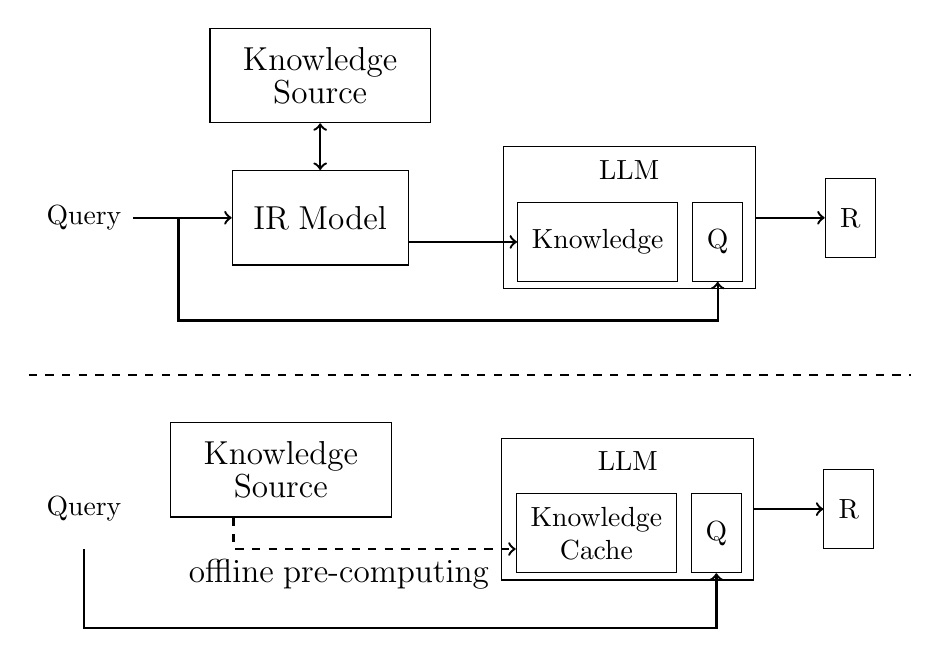
\begin{tikzpicture}[scale=1, transform shape]
    % --- RAG ---

    % IR Model
    \node[
        draw, box, text width=2cm, minimum height=1.2cm, minimum width=2cm, align=center
    ] at (2.5, 1.6) (ir_model) {\large IR Model};
    
    % query on the left of IR Model
    \node[
        text width=1cm, minimum height=1cm, minimum width=1cm, align=center
    ] at ($(ir_model.center) + (-3cm, 0cm)$) (query) {Query};
    % \node at (0, 3) {Query}; 

    % arrow from query to IR Model
    \draw[->, line width=0.3mm] (query) to (ir_model);

    % knowledge source on the top of IR Model
    \node[
        draw, box, text width=2cm, minimum height=1.2cm, minimum width=2.8cm, align=center
    ] at ($(ir_model.north) + (0cm, 1.2cm)$) (knowledge_source) {\large Knowledge Source};
    
    % arrow from knowledge source to IR Model
    \draw[<->, line width=0.3mm] (knowledge_source) to (ir_model);

    % LLM box on the right of IR Model
    \node[
        draw, box, minimum height=1.8cm, minimum width=3.2cm, align=center
    ] at ($(ir_model.east) + (2.8cm, 0cm)$) (LLM_box) {};

    % LLM text on the top of LLM box
    \node at ($(LLM_box.north) + (0cm, -0.3cm)$) (LLM_text) {LLM};

    % knowledge on the bottom of LLM box
    \node[
        draw, box, text width=1.8cm, minimum height=1cm, minimum width=1.8cm, align=center
    ] at ($(LLM_box.south) + (-0.4cm, +0.6cm)$) (knowledge) {Knowledge};

    % arrow from IR Model + (0, -0.3) to knowledge
    \draw[->, line width=0.3mm] ($(ir_model.east) + (0cm, -0.3cm)$) |- (knowledge.west);

    % a q box on the right of knowledge
    \node[
        draw, box, text width=0.4cm, minimum height=1cm, minimum width=0.4cm, align=center
    ] at ($(knowledge.east) + (0.5cm, 0cm)$) (q) {Q};

    % arrow from Query to q, but make it go from buttom to right to top
    \draw[->, line width=0.3mm] 
    ($(query.east) + (1.2cm, 0cm) $) -| ($(query.south) + (1.2cm, -0.8cm)$) -| (q.south);
    % \draw[->] (A.east) |- (B.west);

    % a response box on the right of LLM box
    \node[
        draw, box, text width=0.4cm, minimum height=1cm, minimum width=0.4cm, align=center
    ] at ($(LLM_box.east) + (1.2cm, 0cm)$) (response) {R};

    % arrow from LLM box to response
    \draw[->, line width=0.3mm] (LLM_box.east) to (response);
    
    % --- Seperator between RAG and CAG ---
    \draw[line width=0.3mm, dashed] (-1.2cm, -0.4cm) to (10cm, -0.4cm);

    % --- CAG ---

    % Knowledge Source
    \node[
        draw, box, text width=2cm, minimum height=1.2cm, minimum width=2.8cm, align=center
    ] at (2, -1.6) (knowledge_source) {\large Knowledge Source};
    
    % query on the left of Knowledge Source
    \node[
        text width=1cm, minimum height=1cm, minimum width=1cm, align=center
    ] at ($(knowledge_source.center) + (-2.5cm, -0.5cm)$) (query) {Query};
    % \node at (0, 3) {Query}; 

    % LLM box on the right of knowledge source
    \node[
        draw, box, minimum height=1.8cm, minimum width=3.2cm, align=center
    ] at ($(knowledge_source.east) + (3cm, -0.5cm)$) (LLM_box) {};

    % LLM text on the top of LLM box
    \node at ($(LLM_box.north) + (0cm, -0.3cm)$) (LLM_text) {LLM};

    % knowledge on the bottom of LLM box
    \node[
        draw, box, text width=1.8cm, minimum height=1cm, minimum width=1.8cm, align=center
    ] at ($(LLM_box.south) + (-0.4cm, +0.6cm)$) (knowledge_cache) {Knowledge Cache};

    % arrow from Knowlege Source + (0, -0.3) to knowledge with a explaination text below
    \draw[->, line width=0.3mm, dashed] ($(knowledge_source.south) + (-0.6cm, +0cm)$)
        |- node[text width=4cm, pos=0.7, below] {\large offline pre-computing}
        ($(knowledge_cache.west) + (0cm, -0.2cm)$);

    % a q box on the right of knowledge_cache
    \node[
        draw, box, text width=0.4cm, minimum height=1cm, minimum width=0.4cm, align=center
    ] at ($(knowledge_cache.east) + (0.5cm, 0cm)$) (q) {Q};

    % arrow from Query to q, but make it go from buttom to right to top
    \draw[->, line width=0.3mm] 
    (query.south) -| ($(query.south) + (0cm, -1cm)$) -| (q.south);

    % a response box on the right of LLM box
    \node[
        draw, box, text width=0.4cm, minimum height=1cm, minimum width=0.4cm, align=center
    ] at ($(LLM_box.east) + (1.2cm, 0cm)$) (response) {R};

    % arrow from LLM box to response
    \draw[->, line width=0.3mm] (LLM_box.east) to (response);

\end{tikzpicture}


\end{document}